\subsection{Porous medium}

The above conservation principles are given for single phase systems.
A porous medium, however, consists of multiple phases (fluids such as water, air and non-aqueous phase liquids (NAPLs) as well as solids). 
Moreover, these phases can contain several chemical components which can be dissolved in liquids or adsorbed to the solid phase (Fig. \ref{fig:pm1}).

\vspace{4cm}
\begin{figure}[htbp]
\hspace{3cm}
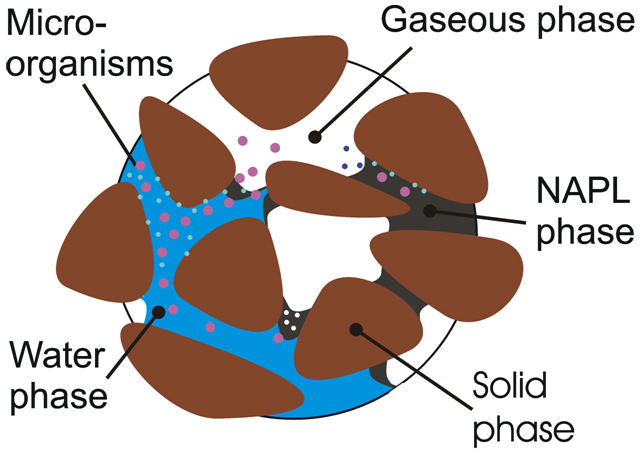
\includegraphics[width=0.06\columnwidth]{figures/pm.png}
\caption{Conceptual approach of a porous medium model}
\label{fig:pm1}
\end{figure}

The macroscopic balance equations are obtained by averaging procedures, normally under the assumption of local thermodynamic equilibrium (e.g. \cite{HasGra:79,Die:85}).
The volume fraction $\epsilon$ of phase $\alpha$ is defined as
%
\begin{eqnarray}
\epsilon^\alpha
= \frac{\Omega^\alpha}{\Omega_0}
\end{eqnarray}

where $\Omega^\alpha$ if the volume of the porous medium occupied by phase $\alpha$ and $\Omega_0$ is the representative elementary volume of the porous medium (REV).
The porosity $n$ of the multi-phase medium is equal to
%
\begin{eqnarray}
\sum_\gamma \epsilon^\gamma
= 
\Porosity
\quad,\quad
\epsilon^s
= \frac{\Omega^s}{\Omega_0}
= 1-\Porosity
\end{eqnarray}

where $\gamma$ is the fluid phase index.
If several fluid phases are present in porous medium they compete for the pore space.
%
Saturation of a fluid phase $\gamma$ is defined as the volumetric
fraction $\VolumetricFraction^\Phase$ related to the sum of all
fluid phases volumetric fractions.
\begin{eqnarray}
\Saturation^\Phase
=
\frac{\VolumetricFraction^\Phase}{\sum_\Phase \VolumetricFraction^\Phase}
\end{eqnarray}

The sum of saturations of all fluid phases must be equal to unity.
\begin{eqnarray}
\sum_\Phase \Saturation^\Phase = 1
\end{eqnarray}

Tab. \ref{tab:conservation_quantities_pm} summarizes the balance quantities for mass, momentum, and energy conservation in a multi-phase porous medium. Phenomenological relationships concerning the fluxes have to be introduced, e.g. Darcy's and Fourier's laws, in order to close the balance equations.
%(see sec. \ref{sec:constitutive_equations_fluxes}).

%
\begin{table}[htb!]
\caption{Balance quantities of a porous medium}
\label{tab:conservation_quantities_pm}
\begin{center}
\begin{tabular}{|l||l|l|}
\hline
Quantity & $\psi$                                  & $\Phi$ \\
\hline
\hline
Mass     & $\epsilon^\gamma \rho^\gamma$           & Fick's law $\epsilon^\gamma \rho^\gamma \v^\gamma$ \\
\hline
Momentum & $\epsilon^\gamma \rho^\gamma \v^\gamma$ & Darcy's law, $\sigma^s$ \\
\hline
Energy   & $\epsilon^\gamma \rho^\gamma e$         & Fourier's law \\
\hline
\end{tabular}
\end{center}
\end{table}
%

% Formulations
There are four unknown field functions to determine:
gas pressure $\Pressure^g$,
water pressure $\Pressure^w$,
solid displacements $\Disp$ and
equilibrium temperature $\Temperature$.
%
In general there are two basic approaches to formulate the balance equations: phase and componental approaches.
%
For non-isothermal processes in partially saturated porous media,
it is more convenient to separate
dry air and vapour masses,
and formulate a mass balance equation for both liquid species,
i.e. liquid and liquid vapour (Gawin et al. 1995, see Chapter 16).

Concept for formulations:
compositional or phase-related approach.
The first approach consists of balancing the species
rather than the phases.
The componental approach is adopted to establish the mass balance equations.

%.........................................................................
% Tabelle als Gleitumgebung
\begin{table}[htb!]
\caption{Primary variables}
\label{tab:}
\begin{center}
\begin{tabular}{|l||l|l|l|l|l||l|}
\hline
aqueous phase   & $\Pressure^w$ & $\Pressure^{gw}$  & $\CapillaryPressure$ & $\Density^w$ & $\Saturation^w$ & $T^w$ \\
gaseous phase   & $\Pressure^g$ & $\Pressure^{ga}$  &                      &              & $\Saturation^g$ & $T^g$ \\
solid   phase   & $\Disp$       &                   &                      &              &    & $T^s$\\
\hline
\end{tabular}
\end{center}
\end{table}
%

All combinations of these primary variables
uniquely describe the states of liquid water, water vapour, gas,
